\documentclass[11pt,a4paper]{article}
\usepackage{fontspec}
\usepackage{polyglossia}
\setdefaultlanguage{russian}
\setmainfont{PT Serif}
\setsansfont{PT Sans}
\setmonofont{Menlo}[Scale=0.85]
\newfontfamily\cyrillicfont{PT Serif}
\newfontfamily\cyrillicfontsf{PT Sans}
\newfontfamily\cyrillicfonttt{Menlo}[Scale=0.85]
\usepackage[margin=2.2cm]{geometry}
\usepackage{amsmath,amssymb}
\usepackage{graphicx}
\usepackage{booktabs}
\usepackage{float}
\usepackage[section]{placeins}
\usepackage{caption}
\usepackage{fancyvrb}
\usepackage[hidelinks]{hyperref}
\graphicspath{{../results/}}
\captionsetup{font=small,labelsep=period}
\setlength{\parskip}{0.4em}
\setlength{\emergencystretch}{3em}

\makeatletter
\let\inputrows\@@input
\makeatother
\newcommand{\student}{Хроян Георгий Овикович, группа 609}

\title{Суперкомпьютерное моделирование и технологии\\[0.3em]
\large Задание 1, вариант 18. Этап 1: OpenMP-программа}
\author{\student}
\date{Октябрь 2026}

\begin{document}
\maketitle

\section{Постановка задачи}

В области
\[
D = \{(x,y): -1<x,y<1\} \setminus \{(x-1)^2+(y-1)^2 \le 1\}
\]
(квадрат без четверти круга с центром в $(1,1)$) требуется приближённо решить задачу Дирихле
\[
-\Delta u = 1, \quad (x,y)\in D, \qquad u = \sin(x+y), \quad (x,y)\in\gamma = \partial D.
\]

\textbf{Метод фиктивных областей.} Задача заменяется задачей в квадрате $\Pi=(-1,1)^2$:
\[
-\Delta v + Q(x,y)\,(v - v_0) = F(x,y), \qquad v\big|_{\partial\Pi} = v_0, \qquad v_0 = \sin(x+y),
\]
где $Q=0$, $F=1$ в $D$ и $Q=1/\varepsilon^2$, $F=0$ в фиктивной области $\hat D = \Pi\setminus\overline D$;
$\varepsilon = h^2$, $h=\max(h_1,h_2)$. В $\hat D$ большой коэффициент $Q$ прижимает решение к $v_0$,
и граничное условие на дуге выполняется приближённо без явного задания границы.

\textbf{Разностная схема.} Сетка $x_i=-1+ih_1$, $y_j=-1+jh_2$, $h_1=2/M$, $h_2=2/N$. Во внутренних узлах
\[
-w_{\bar x x,ij} - w_{\bar y y,ij} + Q_{ij} w_{ij} = F_{ij} + Q_{ij} v_0(x_i,y_j),
\]
на границе квадрата $w_{ij}=v_0(x_i,y_j)$. Коэффициенты усредняются по клетке
$\Pi_{ij}=[x_i\pm h_1/2]\times[y_j\pm h_2/2]$: при доле площади клетки внутри $D$, равной
$s_{ij} = \operatorname{mes}(\Pi_{ij}\cap D)/(h_1h_2)$, получаем $F_{ij}=s_{ij}$,
$Q_{ij}=(1-s_{ij})/\varepsilon^2$. Площадь пересечения клетки с кругом вычисляется точно
(через первообразную $\sqrt{R^2-x^2}$ и включение-исключение по углам клетки).

\textbf{Метод решения.} Метод сопряжённых градиентов с диагональным предобуславливателем
$D_{ij} = 2/h_1^2+2/h_2^2+Q_{ij}$, начальное приближение $w^{(0)}=0$, скалярное произведение
$(u,v)=\sum h_1h_2u_{ij}v_{ij}$, остановка при $\|w^{(k+1)}-w^{(k)}\|_E<\delta=10^{-6}$,
не более $(M-1)(N-1)$ итераций.

\section{Последовательная программа}

Сеточные функции хранятся одномерными массивами размера $(M+1)(N+1)$, узел $(i,j)$ имеет индекс
$i(N+1)+j$. Граничные узлы содержат $v_0$ и не меняются; невязка, направление и $A p$ на границе
равны нулю. Одна итерация CG — три прохода по сетке: вычисление $Ap$ вместе с $(Ap,p)$ и $(p,p)$;
обновление $w$, $r$ вместе с новым $(z,r)$; новое направление $p=z+\beta p$.

Последовательная версия прошла четыре попытки на Polus (каталог \texttt{01\_serial/runs}):

\begin{table}[htbp]
\centering\small
\caption{История последовательной версии на Polus.}
\begin{tabular}{@{}cp{8.2cm}cc@{}}
\toprule
№ & Изменение & Итерации, $80\times80$ & Время, с, $800\times1200$ \\
\midrule
1 & без предобуславливателя, $Q$ и $F$ по узлу & 305 & — \\
2 & + диагональный предобуславливатель & 168 & — \\
3 & + точная площадь клетки (совпадение с эталоном) & 167 & 29.98 \\
4 & + один блок памяти со сдвигом, готовая диагональ & 167 & 17.74 \\
\bottomrule
\end{tabular}
\end{table}

В попытке 3 на Polus программа оказалась в 12 раз медленнее, чем на ноутбуке, при той же скорости
на ноутбуке у прошлой версии кода. С помощью ИИ-ассистента (Claude) была выдвинута гипотеза
о конфликтах в кэше: пять массивов, выделенных отдельно, имели одинаковое выравнивание, и элементы
с одним индексом попадали в одни наборы кэша L1 (64~КБ) ядра POWER8. Размещение массивов в одном
блоке со сдвигом 13~КБ между ними и хранение готовой диагонали ускорили программу в 1.7 раза.

\section{OpenMP-программа}

Пять циклов по узлам сетки (подготовка коэффициентов, старт CG и три цикла итерации) размечены
директивой \texttt{parallel for}: строки $i$ делятся между нитями поровну. Скалярные произведения
считаются через \texttt{reduction}, каждая нить копит свою частичную сумму:

\begin{Verbatim}[fontsize=\footnotesize,frame=single,framesep=2mm]
#pragma omp parallel for reduction(+:pAp, pp)
for (int i = 1; i < M; i++)
    for (int j = 1; j < N; j++) {
        int k = i * s + j;
        Ap[k] = D[k] * p[k] - ih1 * (p[k - s] + p[k + s]) - ih2 * (p[k - 1] + p[k + 1]);
        pAp += Ap[k] * p[k];
        pp += p[k] * p[k];
    }
\end{Verbatim}

Итерации CG выполняются последовательно; $\alpha$, $\beta$ и проверка остановки вычисляются одной
нитью между параллельными циклами. Нити привязаны к ядрам переменной окружения \texttt{GOMP\_CPU\_\allowbreak AFFINITY}
(GCC 4.8.5 на Polus не поддерживает \texttt{OMP\_PLACES}): каждая нить — на первый аппаратный поток
своего ядра; задача занимает узел целиком (\texttt{\#BSUB -x}, 16 ядер POWER8). При 32 нитях — по две
нити на ядро.

\textbf{История попыток} (каталог \texttt{02\_openmp/runs}):
\begin{enumerate}
\item \texttt{parallel for} без \texttt{reduction}: гонка данных на суммах, на 4 и 16 нитях метод
не сходится (лимит 6241 итерация, $w(0,0)$ до $-9\cdot10^8$).
\item \texttt{reduction}: решение верное, но на $400\times600$ ускорение лишь $\times4.9$ на 16 нитях.
\item привязка нитей к ядрам и эксклюзивный узел: $\times12.5$ на 16 нитях (рис.~\ref{fig:binding}).
\end{enumerate}

\begin{figure}[htbp]
\centering
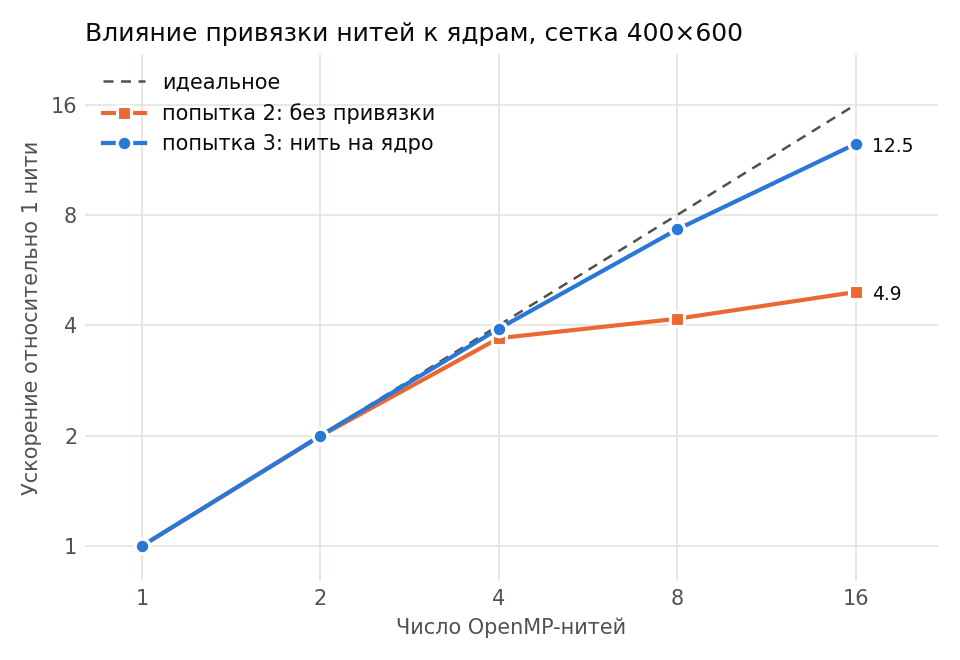
\includegraphics[width=0.66\textwidth]{binding.png}
\caption{Ускорение на сетке $400\times600$ без привязки нитей (попытка 2) и с привязкой (попытка 3).}
\label{fig:binding}
\end{figure}

\section{Результаты}

Все расчёты выполнены на IBM Polus в одном задании на эксклюзивном узле, каждая конфигурация
дважды, в таблицах — минимальное время. Ускорение $S = T_{\text{serial}}/T_{\text{OpenMP}}$
на той же сетке.

\textbf{Проверка на сетке $80\times80$} (табл.~\ref{tab:t80}).

\begin{table}[htbp]
\centering\small
\caption{OpenMP против последовательной программы, сетка $80\times80$.}
\label{tab:t80}
\begin{tabular}{@{}cccccc@{}}
\toprule
Нити & Итерации & Время, с & Ускорение & $w(0,0)$ & $|w-w_{\text{serial}}|$ \\
\midrule
\inputrows ../results/t80_rows.tex
\bottomrule
\end{tabular}
\end{table}

Решение OpenMP-программы совпадает с последовательным на любом числе нитей. На сетке $80\times80$
мало работы, и накладные расходы на запуск и синхронизацию нитей сравнимы с вычислениями,
поэтому 16 нитей медленнее 4.

Время последовательной программы, относительно которого считается ускорение, приведено
в табл.~\ref{tab:serial}, результаты OpenMP-программы — в табл.~\ref{tab:omp} и на рис.~\ref{fig:speedup}.

\begin{table}[htbp]
\centering\small
\caption{Последовательная программа (база для ускорения).}
\label{tab:serial}
\begin{tabular}{@{}cccc@{}}
\toprule
Сетка $M\times N$ & Итерации & Время, с & $w(0,0)$ \\
\midrule
\inputrows ../results/serial_rows.tex
\bottomrule
\end{tabular}
\end{table}

\begin{table}[htbp]
\centering\small
\caption{Результаты расчётов на ПВС IBM Polus (OpenMP-код).}
\label{tab:omp}
\begin{tabular}{@{}ccccc@{}}
\toprule
Нити & Сетка $M\times N$ & Итерации & Время, с & Ускорение \\
\midrule
\inputrows ../results/table1_rows.tex
\bottomrule
\end{tabular}
\end{table}

\begin{figure}[htbp]
\centering
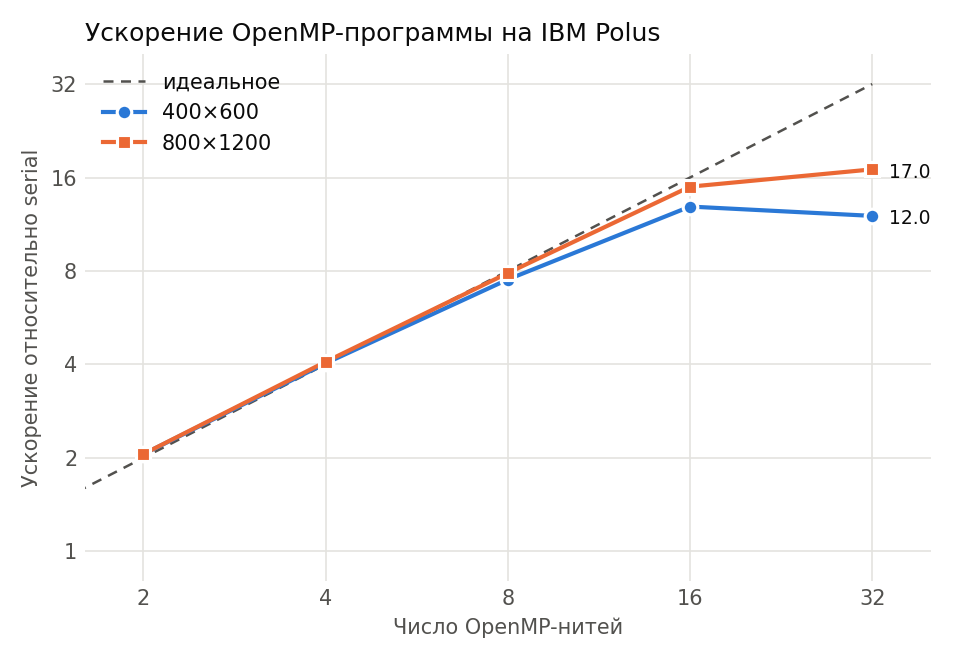
\includegraphics[width=0.66\textwidth]{speedup_omp.png}
\caption{Ускорение OpenMP-программы относительно последовательной.}
\label{fig:speedup}
\end{figure}

\begin{figure}[htbp]
\centering
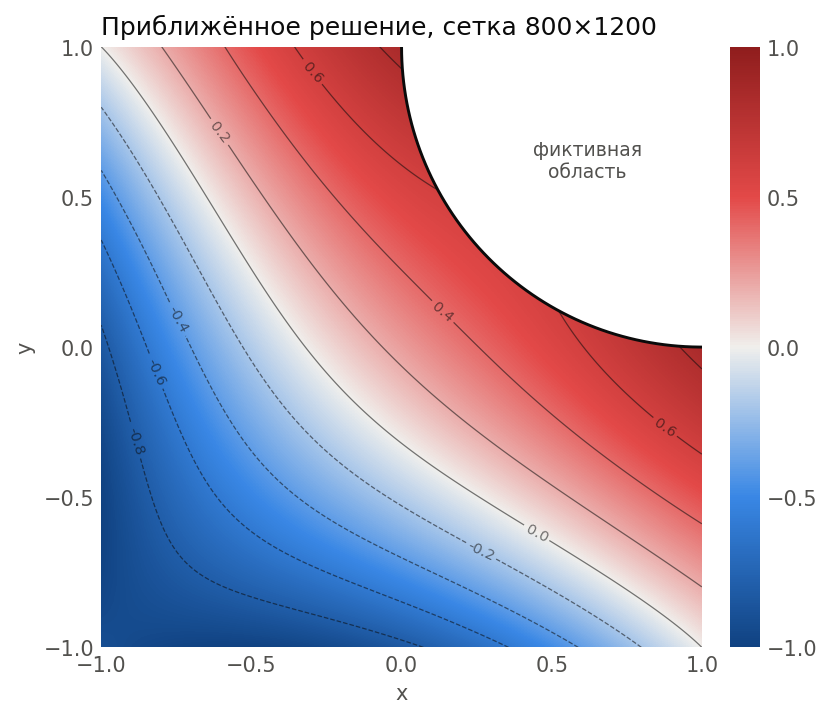
\includegraphics[width=0.56\textwidth]{solution.png}
\caption{Приближённое решение на сетке $800\times1200$; фиктивная область не показана, дуга — граница $\gamma$.}
\label{fig:solution}
\end{figure}

\textbf{Сравнение сеток} (рис.~\ref{fig:solution}–\ref{fig:convergence}). На грубых сетках видна ступенчатая аппроксимация дуги $\gamma$ клетками
сетки; при сгущении граница сглаживается, а значение $w(0,0)$ устанавливается около $0.2432$.
Немонотонность на грубых сетках объясняется тем, что ошибка метода фиктивных областей зависит
от того, как дуга проходит через клетки, и не убывает строго как $O(h^2)$.

\begin{figure}[htbp]
\centering
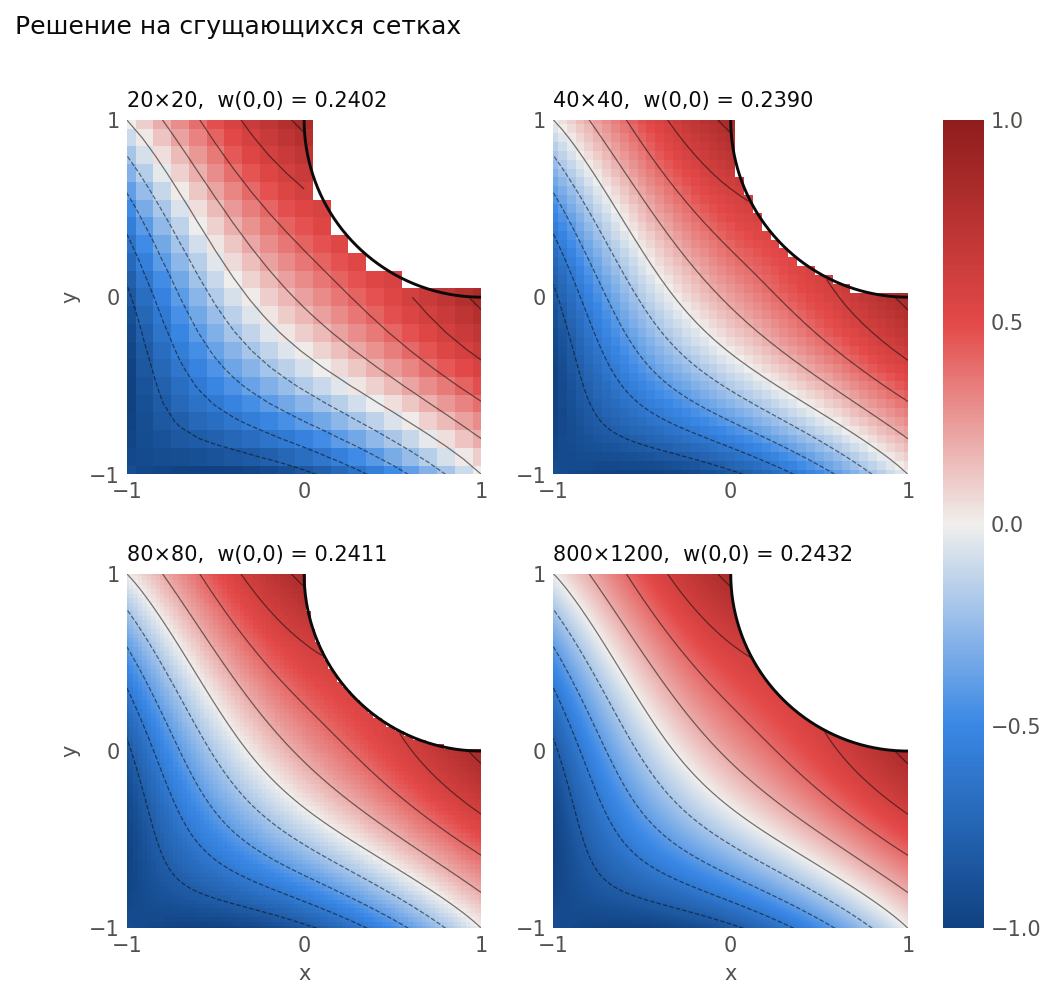
\includegraphics[width=0.72\textwidth]{solution_grids.png}
\caption{Решение на сетках $20\times20$, $40\times40$, $80\times80$ и $800\times1200$ в одной шкале.}
\end{figure}

\begin{figure}[htbp]
\centering
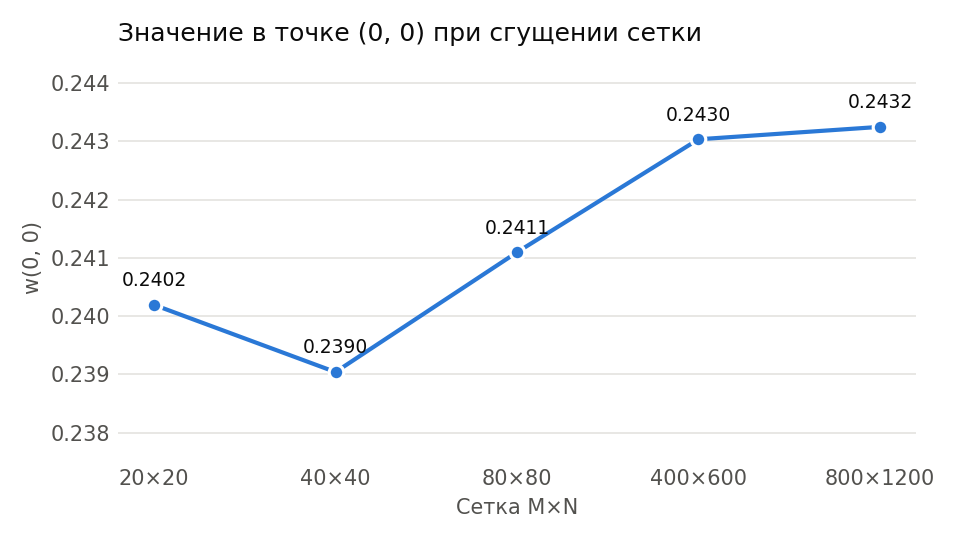
\includegraphics[width=0.7\textwidth]{convergence.png}
\caption{Значение $w(0,0)$ на сгущающихся сетках (последовательная программа, Polus).}
\label{fig:convergence}
\end{figure}

\section{Выводы}

\begin{itemize}
\item Последовательная и OpenMP-программы дают одинаковое решение; на сгущающихся сетках
$w(0,0)$ устанавливается около $0.2432$.
\item До 16 нитей ускорение близко к линейному; на большей сетке оно выше, так как доля
накладных расходов меньше.
\item Две нити на ядро (32 нити на 16 ядрах) на сетке $800\times1200$ дают небольшой прирост
($\times17.0$ против $\times15.0$), а на $400\times600$ замедляют ($\times12.0$ против $\times12.9$):
нити делят вычислительные блоки и кэш ядра, метод ограничен пропускной способностью памяти,
а на меньшей сетке накладные расходы на синхронизацию 32 нитей перевешивают.
\item Решающим для масштабирования оказалась привязка нитей к ядрам: без неё на 16 нитях
ускорение было в 2.5 раза ниже.
\end{itemize}

\end{document}
